\begin{figure}[h]
  \centering
  \setlength{\unitlength}{\columnwidth}
  \begin{picture}(1,0.34)
    \put(0,0){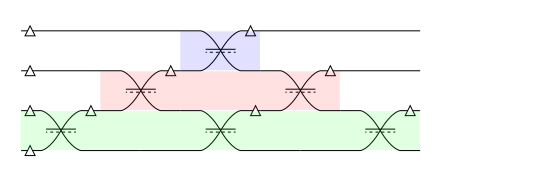
\includegraphics[width=\columnwidth]{figures/example}}
    \put(0.46,0.32){\(r_{4,1}\)}
    \put(0.27,0.22){\(r_{3,1}\)}
    \put(0.66,0.22){\(r_{4,2}\)}
    \put(0.07,0.12){\(r_{2,1}\)}
    \put(0.46,0.12){\(r_{3,2}\)}
    \put(0.85,0.12){\(r_{4,3}\)}
  \end{picture} \\
  \vspace{5mm}
  \includegraphics[width=\columnwidth]{figures/graphs}
  \caption{A \(4 \by 4\) unitary, expressed in linear optics according to the
    scheme in \cite{re-prl-73-58}, and the appropriate \pdf s for choosing
    parameters for a Haar unitary. The reflectivities of the bottom three
    beamsplitters (region (a), shaded green) can be chosen uniformly from the
    interval \(\left[ 0,1 \right)\); those on the second row (region (b),
    shaded red) are chosen from a linear distribution biased towards lower
    reflectivities; and the top one is chosen from a quadratic distribution,
    even more biased towards lower reflectivities.}
  \label{fig:example}
\end{figure}
  
